\section{Background}
This research focuses on increasing the inference speed of transformer models while preserving their generation quality. For this, various experiments affecting the attention mechanism were conducted. This section first describes the standard Multi-Head Attention (MHA) used in the original transformer architecture introduced by Vaswani et al. \cite{vaswani_attention_2017}. Next, the theory behind the optimization techniques (varying kqv-vectors' size, MQA, and GQA) built on top of the standard MHA is explained.

\subsection{Multi-Head Attention (MHA)}
An attention mechanism in transformer models captures context by identifying dependencies between input and output sequences before predicting the next token \cite{vaswani_attention_2017}. Multiple parallel heads within an attention layer enable the model to focus on information from various representation subspaces simultaneously \cite{vaswani_attention_2017}. In other words, each attention head discovers different contextual relationships between the input and the output.

Conceptually, each attention head has its own learnable linear transformation (projection) matrices to transform a token embedding into a key, query, and value ($W_{h_{i}}^{k}, W_{h_{i}}^{q}, W_{h_{i}}^{v}$). Then the attention output is computed for the current query using all previous keys and values for the given head. Each head produces its own attention output, which is then concatenated (with the outputs from all the other heads) and transformed using the output projection matrix $W_O$. Usually, matrices $W_{h_{i}}^{k}, W_{h_{i}}^{q}, W_{h_{i}}^{v}$ from each head are concatenated into one ($W^{k}, W^{q}$, and $W^{v}$ respectively) for convenience and the bigger transformed vectors are split into smaller vectors only later such that each corresponds to each head to calculate respective attention outputs. \textit{Figure \ref{fig:obtaining_key}} visualizes this process of producing a key vector for the batch size of one for simplicity and 4 attention heads. The process for obtaining queries and values is similar except that for value vectors, the dimensionality $d_v$ can differ from $d_k$.

\begin{figure}[htbp] % [htbp] specifies the preferred placement options (here: here, top, bottom, page)
    \centering
    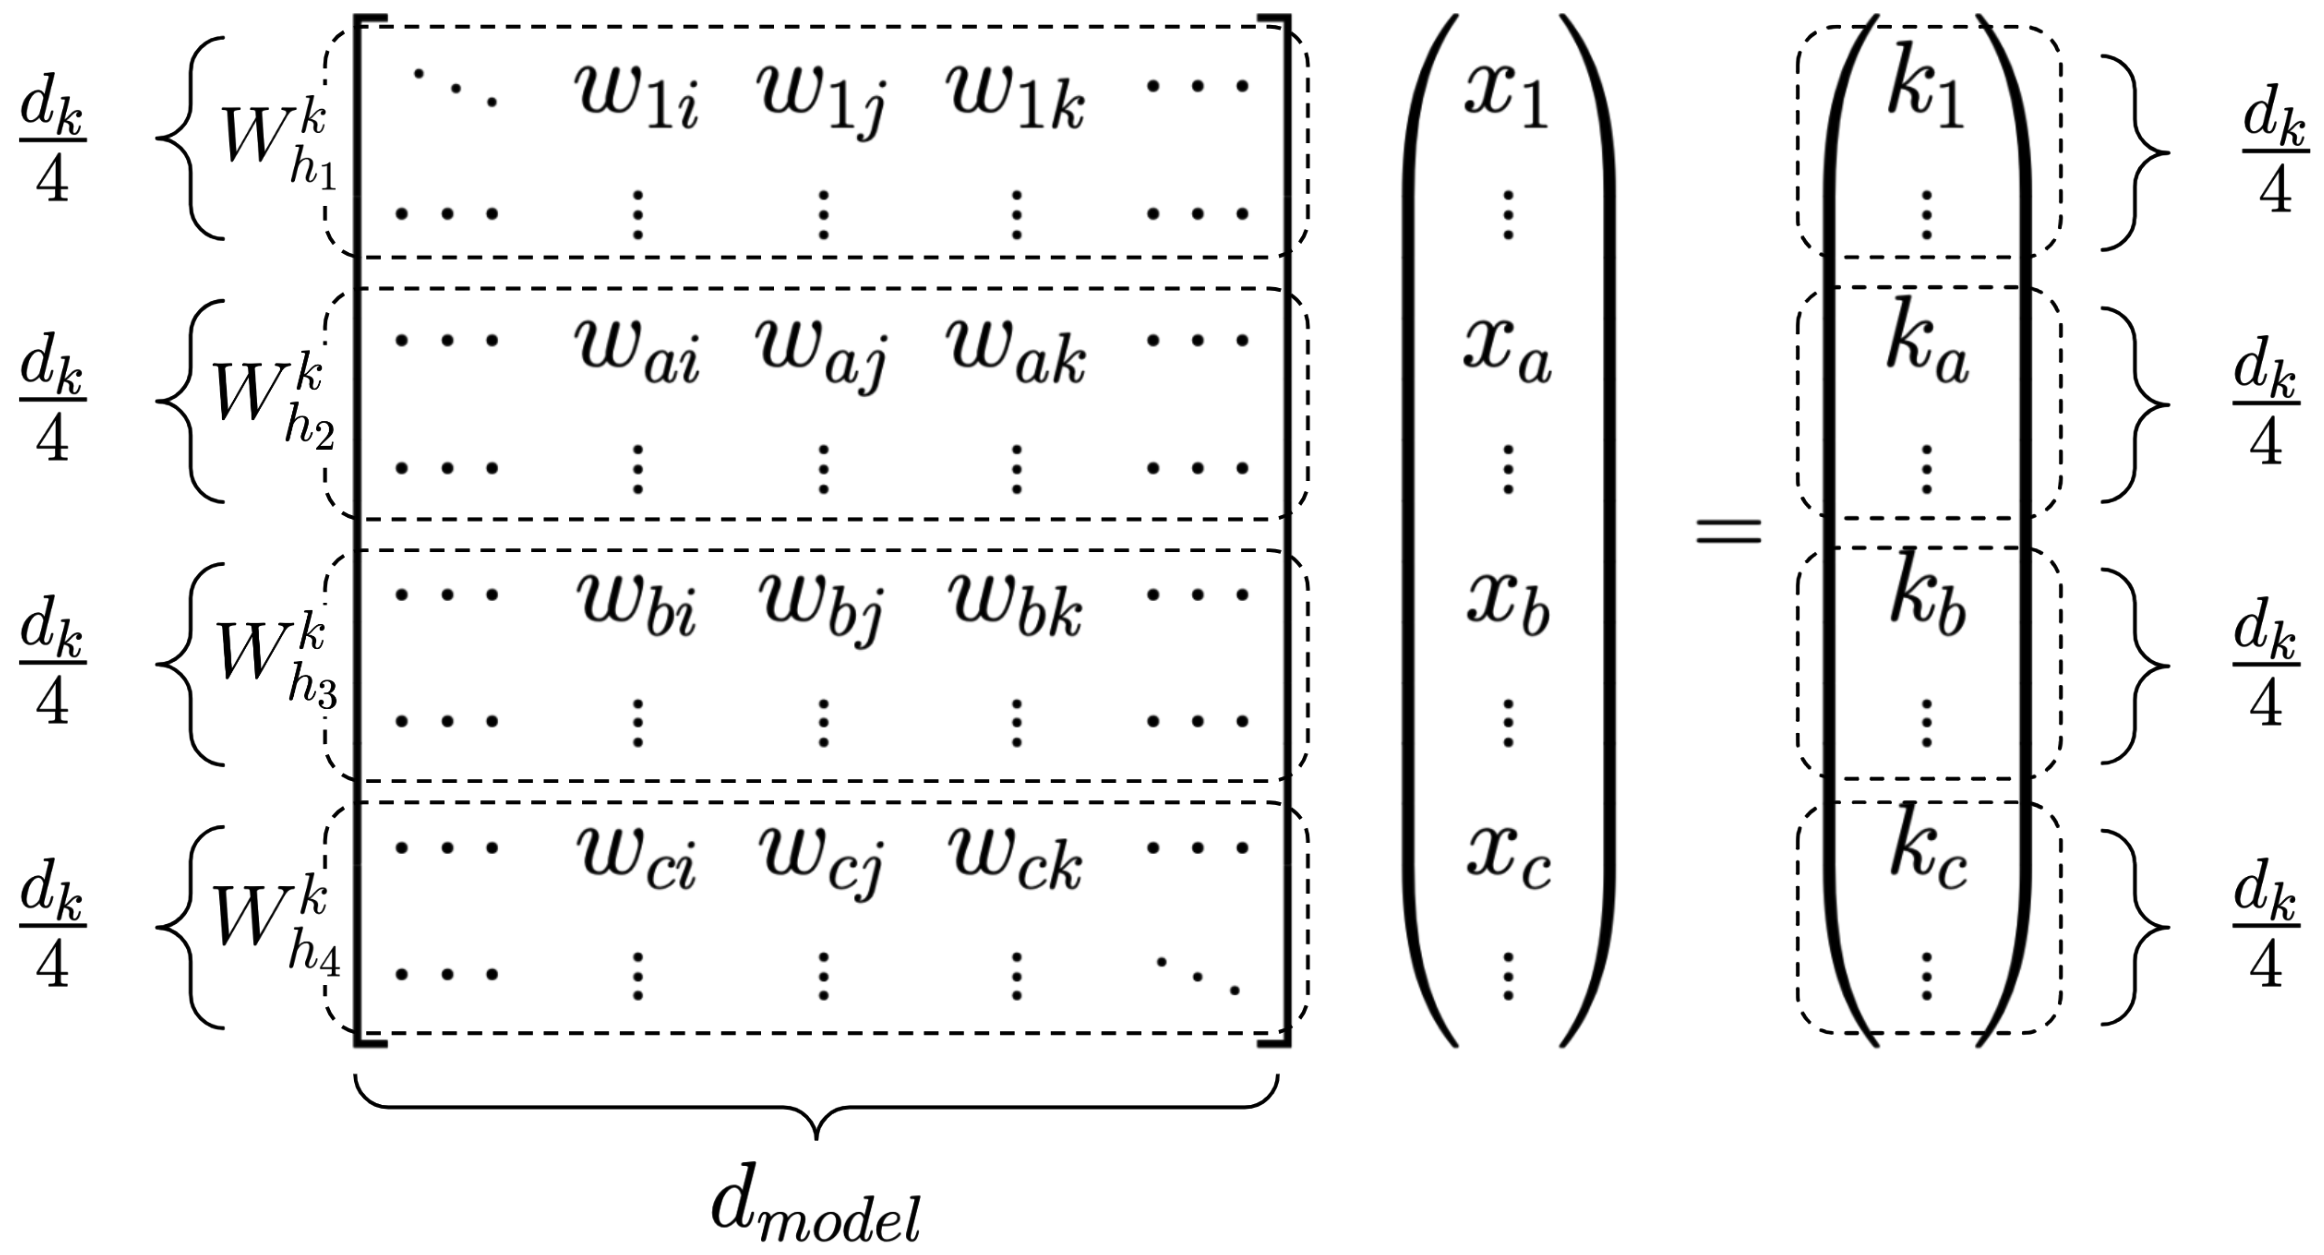
\includegraphics[width=0.5\textwidth]{research paper/images/obtaining_key.png} % Replace "example-image" with the filename of your image
    \captionsetup{justification=centering}
    \caption{Obtaining a key from an embedding vector (for one sequence) in a model with 4 attention heads. $d_{model}$ stands for an embedding dimension (dimension of the vector $x$); $d_k$ is a dimensionality of a key which in this case is equal to $d_{model}$.}
    \label{fig:obtaining_key}
\end{figure}

Once key and value vectors are calculated, they are added to the KV cache such that they can be reused when calculating attention outputs for the next query (as in incremental/autoregressive decoding the next token attends to all the previous ones). The number of keys and values in the cache is capped at the context window size.   

To calculate attention outputs for one attention head according to the procedure described by Vaswani et al. \cite{vaswani_attention_2017}, we first retrieve all the keys and values from the cache to obtain $K$ and $V$ tensors. If several batches are processed in parallel, the vector $x$ will become a tensor $X$; $K$ and $V$ tensors will be extended by one extra dimension equal to the number of batches; and the query vector $q$ will then become a tensor $Q$. Then, the normalized dot product between $Q$ and $K$ tensors is calculated to find the weights that will be multiplied by tensor $V$ to obtain the final attention outputs.

Once the attention outputs are calculated for each head, the results are concatenated alongside the head dimension before being passed to be transformed by the output projection matrix which is a final step in the mechanism. 


\subsection{A Problem with MHA and Proposed Changes for Inference Optimization}
As mentioned before, to account for all the past tokens, the KV cache stores all the previous keys and values. The cache can take up a lot of memory given that we store key and value vectors for each attention head, for each previous token, and for each sequence in a batch in case we process several inputs in parallel. In incremental decoding the attention mechanism is called each time we generate a token, hence the KV cache will have to be constantly fetched to compute the attention outputs. Given that computation can be parallelized, frequently accessing memory emerges as the primary bottleneck that causes inference slowdowns \cite{pope_efficiently_2022} \cite{shazeer_fast_2019} \cite{williams_roofline_2009}. Thus, the goal is to minimize the ratio of the memory taken by the KV cache (space complexity) relative to the number of computations (time complexity) induced by calling an attention mechanism which effectively comes down to just reducing the KV cache size \cite{shazeer_fast_2019}. 

To achieve the smaller size of a KV cache, one can try the following:
\begin{enumerate}
    \item Reduce the context window size such that we store fewer keys and values;
    \item Reduce the number of sequences in the batch (inputs that we process in parallel);
    \item Reduce the dimensionality of key and value vectors;
    \item Somehow dismiss keys and values stored for certain (selected) attention heads.
\end{enumerate}
Reducing the context window size is not desirable as it will decrease the model's capability to account for context, possibly making it too forgetful and less sophisticated. Furthermore, depending on the application's nature, processing fewer inputs is not always possible and many sequences in a batch can be necessary. Thus, only the last two options are left and are experimented on in this study, the latter of which could be approached as described in the next two subsections.


\subsection{Multi-Query Attention (MQA)}
Multi-Query Attention was introduced by Shazeer \cite{shazeer_fast_2019} and was an initial step to optimizing the inference speed by dismissing keys and values for certain attention heads. Namely, in this approach, keys and values in all heads but one are omitted such that queries from all heads attend to keys and values from only one head. That means that $W^k$ and $W^v$ are reduced to just $W_{h_{1}}^{k}$ and $W_{h_{1}}^{v}$ respectively (\textit{Figure \ref{fig:obtaining_kv_mqa}}). At the same time, $W^q$ remains the same as depicted in \textit{Figure \ref{fig:obtaining_key}} except that the matrix is for query projections.

\begin{figure}[htbp] % [htbp] specifies the preferred placement options (here: here, top, bottom, page)
    \centering
    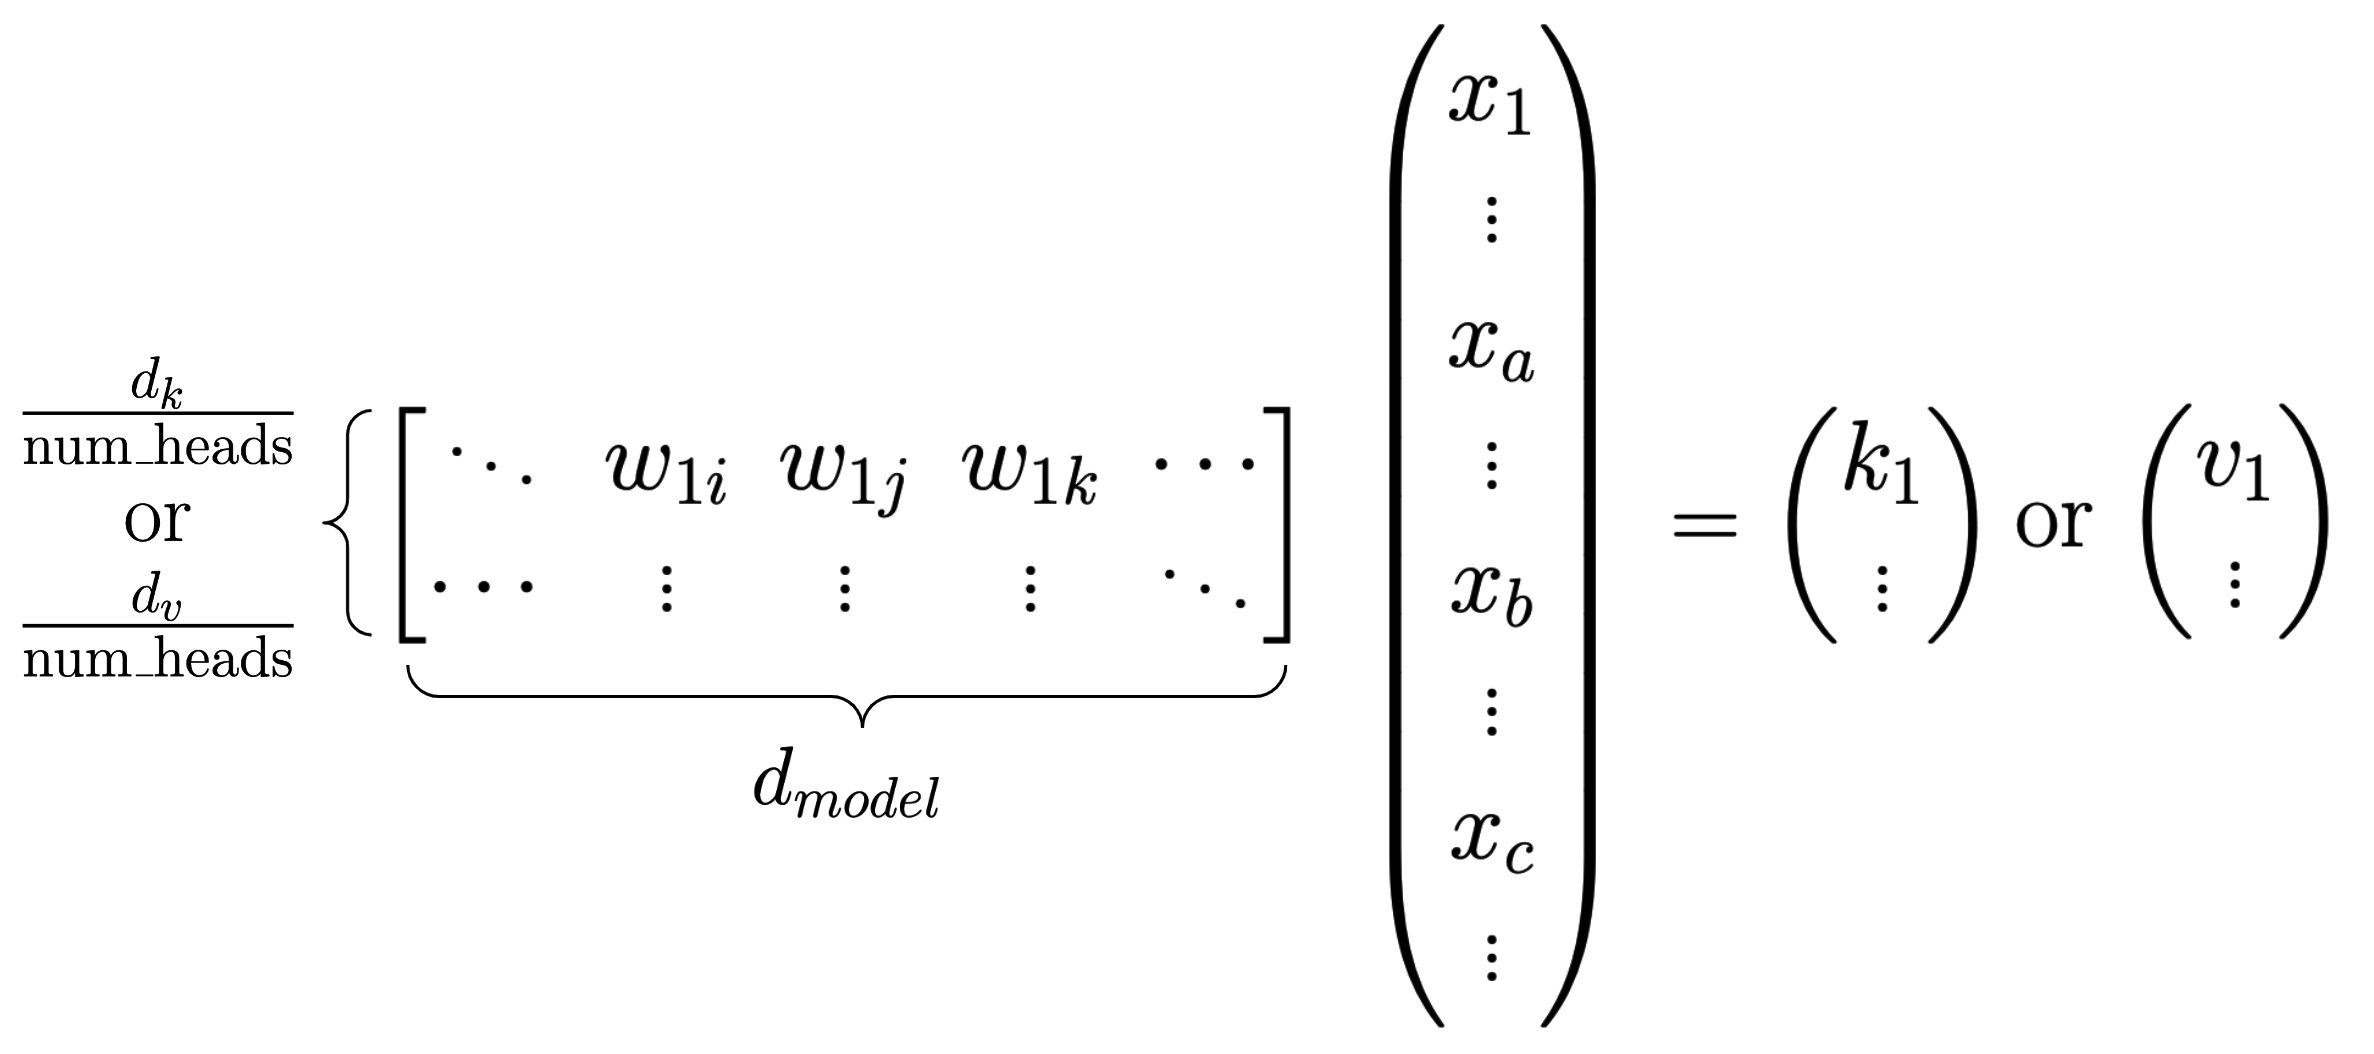
\includegraphics[width=0.5\textwidth]{research paper/images/obtaining_kv_mqa.png} % Replace "example-image" with the filename of your image
    \captionsetup{justification=centering}
    \caption{Obtaining a key OR value from an embedding vector (for one sequence) in MQA with an arbitrary number of attention heads. $d_{model}$ stands for an embedding dimension (dimension of the vector $x$); $d_k$ is a dimensionality of key vectors, $d_v$ - of value vectors.}
    \label{fig:obtaining_kv_mqa}
\end{figure}

As a result, each query vector from each query head attends to key vectors from a single key head multiplied by vectors belonging to a single value head (\textit{Figure 3}). This is equivalent to shrinking the KV cache size by a factor of the total number of attention heads $num\_heads$.

MQA has shown a significant inference speedup when having a large batch size, however, it led to some quality degradation \cite{shazeer_fast_2019}. Moreover, MQA might cause a too-aggressive cut when having a bigger model with a large number of attention heads as the proportion $\frac{1}{num\_heads}$ is too small \cite{ainslie_gqa_2023}. To address this issue, Grouped-Query Attention was introduced by Ainslie et al. \cite{ainslie_gqa_2023}.

\begin{figure}[htbp] % [htbp] specifies the preferred placement options (here: here, top, bottom, page)
    \centering
    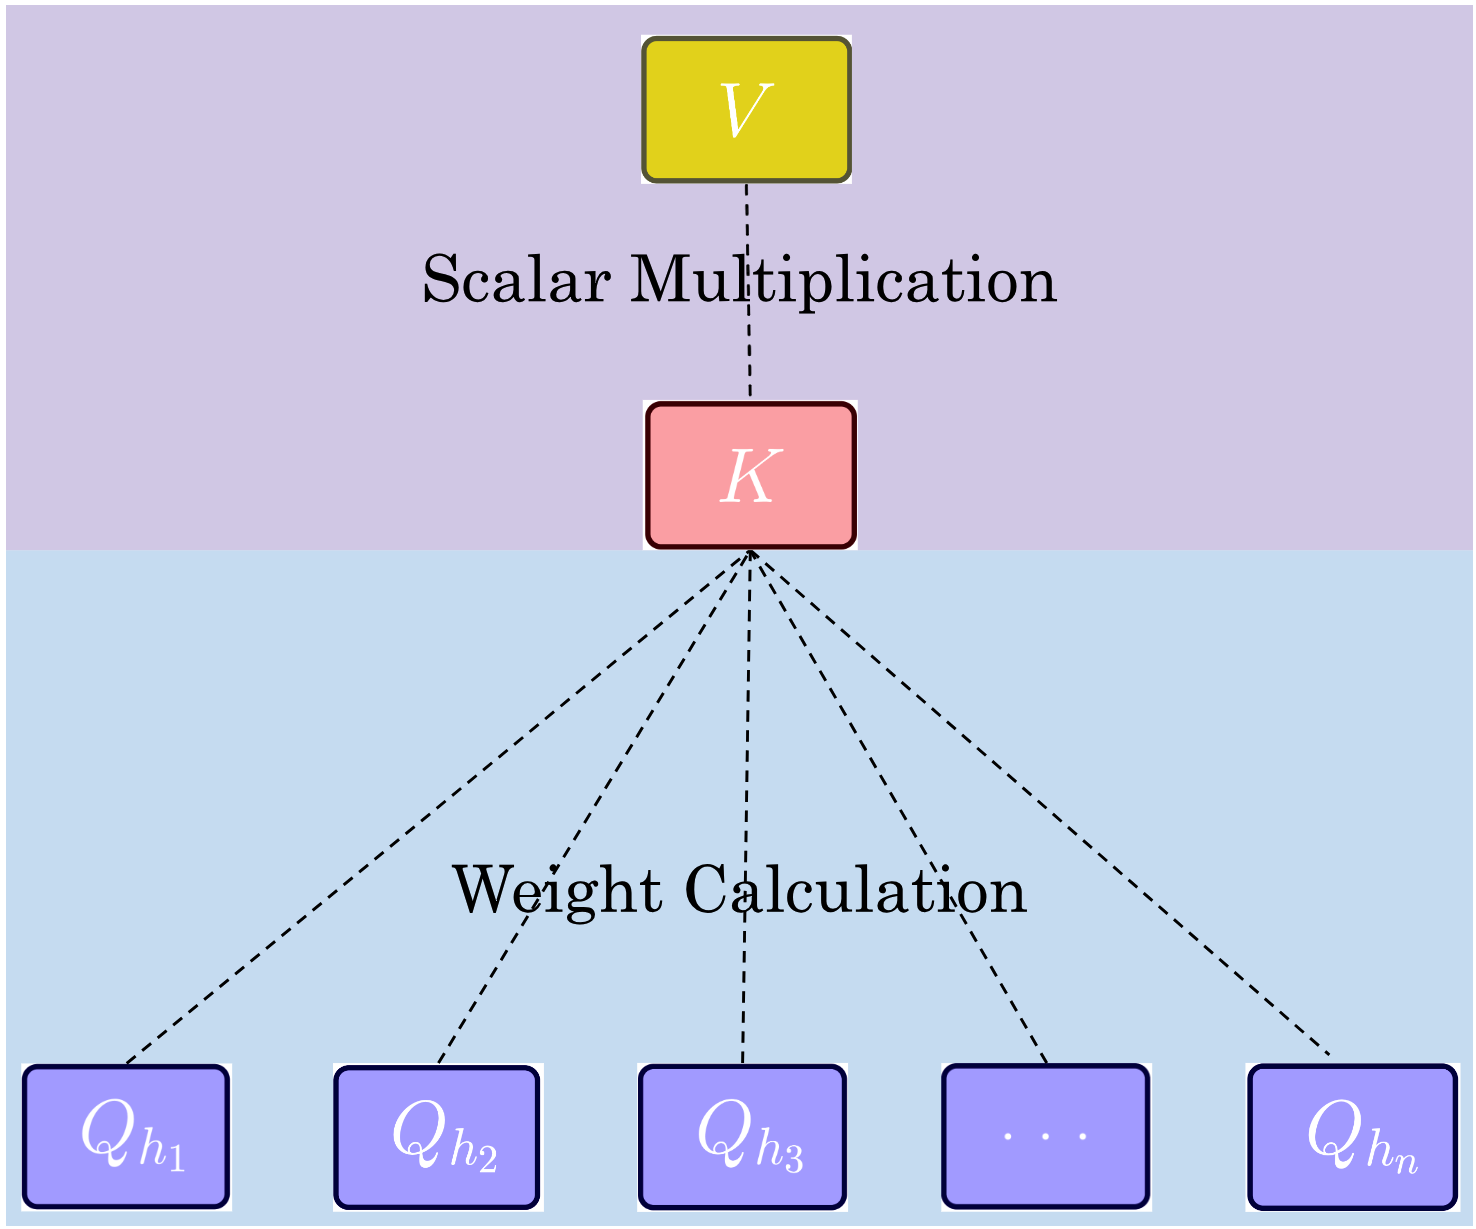
\includegraphics[width=0.5\textwidth]{research paper/images/mqa.png} % Replace "example-image" with the filename of your image
    \captionsetup{justification=centering}
    \caption{MQA visualisation. Inspired by Ainslie et al. \cite{ainslie_gqa_2023}}
    \label{fig:mqa}
\end{figure}
\subsection{Grouped-Query Attention (GQA)}
Grouped-query attention represents a generalization over MQA and is an interpolation between MHA and MQA (including both). Instead of leaving only one key and value head, GQA models have $n$ key-value heads where $n \in [1, num\_heads]$. This is equivalent to grouping some queries around these key-value heads (as we now have more query heads, a group of query heads are those that attend to the same key head). Similarly to MQA, the number of query heads remains equal to the total $num\_heads$. This way, when the model has many attention heads, the proportion of key-value heads to the total number of heads can be preserved, and the quality drop will be less noticeable \cite{ainslie_gqa_2023}. Furthermore, the ability to select the number of key-value heads allows for flexibility in balancing the trade-off between the model's speed and quality. 

\textit{Figure 4} showcases the process of acquiring keys (similarly, for the batch size of 1 for simplicity) in GQA for 4 attention heads and 2 groups. The procedure for obtaining the values is again the same except having a separate learnable transformation matrix and that $d_v$ can be different from $d_k$ based on the model's configuration. For the same number of groups and heads, \textit{Figure 5} demonstrates the process of the attention output calculation.

\textbf{Figures 4 and 5 are in the making...}

% \begin{itemize}
%     \item Explain how Multi-Head Attention works in decoders
%     \item Explain why reducing the size of key and value tensors is important in autoregressive decoding \cite{pope_efficiently_2022} \cite{shazeer_fast_2019} \cite{williams_roofline_2009} conceptually and using time/space complexity
%     \item Explain what is MQA \cite{shazeer_fast_2019}
%     \item Explain what is GQA and include a figure showcasing all three \cite{ainslie_gqa_2023}
%     \item Mention the goal of reducing key and value vector sizes and that in the MQA paper it's not investigated properly 
%     \item Mention again that GQA experiment used uptrained models and here we recreate it using pre-trained models
%     \item Mention that no one tested yet how do MQA and GQA behave when given different number of attention heads (maybe \cite{michel_are_2019}) 
% \end{itemize}

% Transformers is a state-of-the-art deep learning architecture in large language models used for data processing (encoding) and data generation tasks (decoding) \cite{vaswani_attention_2017}. Over time, transformer models have been scaled to enormous sizes with hundreds of billions of parameters to improve performance. This made the models less sustainable and more expensive both to train and operate due to the computational requirements induced by the scaling. 

% For this reason, the TinyStories dataset has specifically been designed to demonstrate the capability of improving the models' sample efficiency. It has been shown that improving the sample efficiency can significantly reduce the number of parameters while preserving the model's ability to generate coherent, diverse, and consistent results with the model demonstrating some reasoning capabilities \cite{eldan_tinystories_2023}. To facilitate the sample efficiency in models, the TinyStories was designed to be more cohesive and suitable for learning English grammar and vocabulary.

% Furthermore, the research reveals that the smaller models exhibit similar behaviour to their larger counterparts when it comes to architectural decisions \cite{eldan_tinystories_2023}. This, coupled with their suitability for limited-resources environments, positions them as ideal platforms for architectural experimentation in scenarios with restricted access to data and computational resources. 

% For some types of work in computer science the methodology is standard: analyze the problem (e.g., make assumptions and derive properties), present a new algorithm and its theoretical background, proving its correctness, and evaluate unproven aspects in simulation.
% Then an explanation of the methodology is often omitted, and the setup of the evaluation is part of a later section on the evaluation of the ideas.\footnote{This already shows that there is no single outline to be given for all papers.}
% In this case, explain relevant (background) concepts, theory and models in this section (with references) and relate them to your research question.
% Also this section then typically contains a more precise, formal description of the problem.

% Do not forget to give this section another name, for example after the problem you are solving.
